\section{建系法探究空间关系}

% \tdplotsetmaincoords{80}{105}

% \begin{tikzpicture}[tdplot_main_coords, scale=1.5, font=\sansmath\sffamily]
%     % 定义正方体的边长
%     \pgfmathsetmacro{\s}{3}

%     % 定义8个顶点坐标
%     % 为了匹配图片视角，我们将隐藏的D点设为原点
%     \coordinate (D) at (0,0,0);
%     \coordinate (A) at (\s,0,0);
%     \coordinate (C) at (0,\s,0);
%     \coordinate (B) at (\s,\s,0);
%     \coordinate (D1) at (0,0,\s);
%     \coordinate (A1) at (\s,0,\s);
%     \coordinate (C1) at (0,\s,\s);
%     \coordinate (B1) at (\s,\s,\s);

%     % 绘制隐藏的边 (虚线)
%     \draw[dashed, thick] (D) -- (A);
%     \draw[dashed, thick] (D) -- (C);
%     \draw[dashed, thick] (D) -- (D1);

%     % 绘制可见的边 (实线)
%     \draw[thick] (A) -- (B) -- (C);
%     \draw[thick] (A) -- (A1);
%     \draw[thick] (B) -- (B1);
%     \draw[thick] (C) -- (C1);
%     \draw[thick] (A1) -- (B1) -- (C1) -- (D1) -- (A1);

%     % 标注顶点
%     \node[below left] at (A) {$A$};
%     \node[below right] at (B) {$B$};
%     \node[below right] at (C) {$C$};
%     \node[below left] at (D) {$D$};
%     \node[above left] at (A1) {$A_1$};
%     \node[above right] at (B1) {$B_1$};
%     \node[above right] at (C1) {$C_1$};
%     \node[above left] at (D1) {$D_1$};
% \end{tikzpicture}

\begin{example}
    正方体 $A B C D-A_1 B_1 C_1 D_1$ 的棱长为 $1, ~ E$ 为棱 $D D_1$ 的中点，点 $P$ 在面对角线 $B C_1$ 上运动（ $P$ 点异于 $B$、$C_1$ 点），以下说法错误的是（ \hspace{2em}）

    \begin{itemize}
        \item $B D_1 / /$ 平面 $A E C$
        \item $A_1 P \perp B_1 D$
        \item 直线 $B_1 E$ 与平面 $C D D_1 C_1$ 所成角的余弦值为 $\frac{2}{3}$
        \item 三棱雉 $P-A C D_1$ 的体积为 $\frac{1}{6}$
    \end{itemize}
\end{example}

\begin{center}
    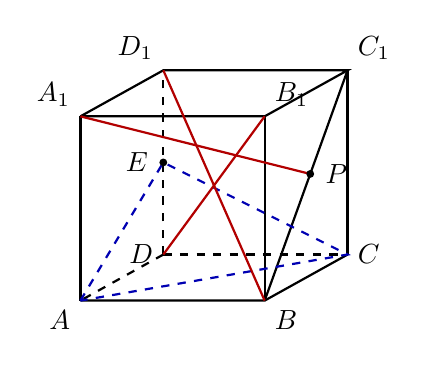
\begin{tikzpicture}[
            scale=0.78,
            x={(1cm,0cm)},
            y={(0.45cm,0.25cm)},
            z={(0cm,1cm)},
            thick,
            point/.style={circle, fill=black, inner sep=1pt}
        ]
        \def\s{3}

        \coordinate (A) at (0,0,0);
        \coordinate (B) at (\s,0,0);
        \coordinate (C) at (\s,\s,0);
        \coordinate (D) at (0,\s,0);
        \coordinate (A1) at (0,0,\s);
        \coordinate (B1) at (\s,0,\s);
        \coordinate (C1) at (\s,\s,\s);
        \coordinate (D1) at (0,\s,\s);
        \coordinate (E) at (0,\s,1.5);
        \coordinate (P) at (\s,1.65,1.65);

        \draw[dashed] (D) -- (A);
        \draw[dashed] (D) -- (C);
        \draw[dashed] (D) -- (D1);
        \draw (A) -- (B) -- (C);
        \draw (A) -- (A1);
        \draw (B) -- (B1);
        \draw (C) -- (C1);
        \draw (A1) -- (B1) -- (C1) -- (D1) -- (A1);
        \draw (B) -- (C1);

        \draw[blue!70!black, thick, dashed] (A) -- (E) -- (C) -- cycle;
        \draw[red!70!black, thick] (B) -- (D1);
        \draw[red!70!black, thick] (A1) -- (P);
        \draw[red!70!black, thick] (B1) -- (D);

        \node[point, label=left:$E$] at (E) {};
        \node[point, label=right:$P$] at (P) {};
        \node[below left] at (A) {$A$};
        \node[below right] at (B) {$B$};
        \node[right] at (C) {$C$};
        \node[left] at (D) {$D$};
        \node[above left] at (A1) {$A_1$};
        \node[above right] at (B1) {$B_1$};
        \node[above right] at (C1) {$C_1$};
        \node[above left] at (D1) {$D_1$};
    \end{tikzpicture}
\end{center}
